\documentclass[a4paper,11pt]{article}

% packages
\usepackage{array}
\usepackage{tabularx}
\usepackage{booktabs}
\usepackage{graphicx}
\usepackage{framed}
\usepackage{comment} % comment multiple lines
\usepackage{spverbatim} % pasting large amounts of texts such as SQL code, and more
\usepackage{alltt}
\usepackage{float}
\usepackage{url} % URLs used for 
\usepackage{hyperref}
\usepackage{fancyhdr}
\usepackage[utf8]{inputenc} % Use UTF 8. This allows æ, ø, å
\usepackage{longtable} % tables over multiple pages
\usepackage{pdfpages} % include PDF
\usepackage{enumitem} % used bu the set list markup
\usepackage[T1]{fontenc} % For writing < and > correctly

% Markup
\setlength{\parskip}{0.5em} % Setting paragraph view
\setlist[itemize]{itemsep=0.1em, topsep=0pt} % Setting distance between items and around item group

% commands
\newcommand{\ra}[1]{\renewcommand{\arraystretch}{#1}} % custom command used for tables
\newcommand{\specialcell}[1]{\begin{tabular}{@{}c@{}#1\end{tabular}}}
\newcommand{\Sh}{\nolinebreak\hspace{-.05em}\raisebox{.6ex}{\tiny\bf \# }}
\newcommand{\pref}[1]{ section \ref{#1}, page~\pageref{#1}}
\newcommand{\apref}[1]{ Appendix,\pref{#1}}
\newcommand{\subsubsubsection}[1]{\paragraph{#1}\mbox{}\\}

% define the author and title for frontpage
\author{Oz}
\title{RentIt}
\pagestyle{fancy}
\begin{document}
\maketitle
\tableofcontents
\newpage

% Inputs
\section{Abstract}
\newpage
\section{Introduction}
This paper was written for the second Year Project: Software Development in Large Teams with International Collaboration at the IT-University of Copenhagen in spring 2013.

The project has been divided into two parts. In the first part we where to developed a web service, while a group from Singapore Management University (from hereon referred to as SMU) was to develop a client using the web service we made. At the second part of the project, we where to develop a client using our web service.

The first part of the project has therefore been very focused on how to collaborate with another group on the other side of the world. A collaboration where both time, culture and language are factors to be kept in mind.

In this paper we will explain our approach to the project and the collaboration in the first part.
The paper is divided into two primary parts, the implementation of the server and the implementation of the client.
The two parts should be able to be read independently, with only few significant references between. We will end each part with a reflection and a conclusion of the work made in this part.
At the end of the paper we will conclude on the entire project.
\newpage
\section{Introduction to collaboration with SMU}
In this project we had the amazing opportunity to collaborate with a group of students from the Singapore Management University.

The collaboration was started with a short video chat in order to say hello and trade first impressions. We held two video chat meetings each week for the rest of the project.

In the beginning both parties made sure to formulate sentences very clearly and straight forward, trying not to say something that could be perceived with a different meaning than intended. We found that communicating via text was way easier as the accent was no factor.
With support from text every meeting became easier and more loose, and the conversation became natural with their best English speaker.

From our group we chose Claus as our liaison and they chose Lynette. They were the ones mainly responsible for communication between the groups and for keeping their own group well-informed.

We were aware of the fact that our Singaporean group was of a different culture and that they might conceive something differently than we would. Fortunately it did not turn out to be a problem though.

Singapore is 7 hours ahead of Denmark during daylight saving time and 8 hours when not. We usually held our meetings around noon Danish time, which is late afternoon Singaporean time. It was not hard to arrange meetings, but the time difference often made for long response times.

By the end of our collaboration each member from each group reflected upon the whole process. The reflections can be found on our shared wiki and in our appendix.

Our shared wiki page can be found in the appendix and at: \textbf{[ TODO: Reference (M) ]}
\\\url{wiki.smu.edu.sg/is411/User:Team7}

Their website can be found at:
\\\url{http://green.smu.edu.sg/gspm2013/team07/}
\newpage
\section{Chosen technologies}
In the very beginning, even before our collaboration with SMU we decided upon which technologies we would like to use. Later, we had the parts concerning SMU approved by them.

We chose to use F\Sh for developing our server. We had all recently been introduced to the programming language and were very exited about it and the completely different ideas on which it is based. We all attended a course in the language, but wanted to use it in a bigger project in order to put it into perspective, and so we unanimously decided it as the language of choice for our server, which was approved by our lecturer.

For SMU to be able to use our server we had to expose the functionality as a web service. Two different technologies were at hand, namely SOAP and REST. We chose to use REST because we believe it is much simpler than using SOAP and thereby less time consuming for us to use in the client.

We faced some difficulties in exposing the web service as we chose to use F\Sh, however. We learned that the Windows Communication Foundation for making web services in F\Sh was not in a state that was easy for us to use, and therefore we planned to implement a thin service layer in C\Sh with the responsibility of forwarding requests to the F\Sh code. This, however, turned out not to be so thin as we planned.

For storing data we all agreed to use a relational database supporting SQL. We all used this before with great success and wanted to keep using it.
Having made this decision we had to choose between two different implementations which would be available in the deployed environmen: MySQL and MSSQL. We started out by agreeing on using MySQL, as we all had worked with it before, and favored it to MSSQL. We also talked to our lecturer about this and he was indifferent about it. However, when we started making our data model, and deployed it on the server it became apparent that it was easier to use MSSQL, as we did not need to setup the server in any way.

Lastly we decided on which technology we wanted to write our own client in. We did not want to program our client in ASP, or any of the other Microsoft web languages. Some of us had experience with PHP, and one in the group had extensive experience with it. We decided that we wanted to try programming our client in object oriented PHP. We asked our lecturer, and it was approved.
\newpage
\section{Target audience}
We tried to make our back-end server and data model as flexible and capable as possible. We wanted it work with whatever audience one might choose to target with ones client. We chose to do so, though it is time consuming, because we did not want it set any limits to any client which wanted to use our service. We also had in mind that both we and our Singaporean group was going to use the service and we did not know what sort of site they had in mind.

For our client we really wanted to do something like Netflix, but without the limitations of only video content. 
\\We see our target content providers as companies who cheaply wants to make content available for the masses and we want to make it up to the providers to set the price and to decided how much money they want to earn, if any at all.
\\To make our client attractive for content providers we wanted to support both free products, paid products as well as products for rent. 

We expect to make earnings from commercials and by feeing content providers per sale. But one should keep in mind that our service relies heavily on its content and its content providers, as many similar services does and our competition is strong.

Limitations

Our very wide choice of target audience might prove not to be lucrative. Netflix is a very specific service and people know exactly what they can get from that service. Our wide array of services does not limit us, per se, but a more simple service can focus stronger on its target and there by hit more accurately.
\newpage
\section{Server}
\subsection{Planning}
This section explains the rationale behind the decisions we took regarding everything but the actual server implementation.
\subsubsection{User types}
\todo{Quite sudden to be talking about this}{Michael}
\label{s_actor-goal-list}
Below we give an overview of the functionality the server should provide to each dynamically defined user type that we have chosen for this version of the server. \todo{Det er da ikke hvad det afsnit skal gøre?}{k}

\begin{description}
	\item [Non-registered user] \hfill \\
		This is the user type with the least options, only being able to browse the products and register to become a customer.
	\item [Customer]  \hfill \\
		The customer is quite possibly the most common user type the service will have. The big difference between a customer and a non-registered user is the customer's ability to:
		\begin{itemize}
			\item buy/rent products
			\item buy credits
			\item download/view products
			\item rate products
		\end{itemize}
	\item [Content provider] \hfill \\
		The content provider is, as the name suggest, the kind of user who will be filling the service with products. They cannot rent, buy, or rate products, only upload and manage their own products. \todo{not true}{Claus} \todo{True during planning phase}{Michael}
	\item [Admin] \hfill \\
		The admin is the most powerful user type with the power to administrate any registered user or product, including changing any piece of associated information.
\end{description}
\subsubsection{Use Cases}
In the following the use cases for the server will be presented. This gives an explanation of which functionality the server should offer, and to whom (that is which user types).
\label{s_actor-goal-list}
In the system we have four kinds of actors:
\begin{description}
	\item [Non-registered user] \hfill \\
		This is the user type with the least options. Only allowed to browse the products, and register to become a registered user.
	\item [Customer]  \hfill \\
		This is the customer, the consumer, and quite possible the most common user type the service will have. The differences between a registered and a non-registered user is that the registered user is able to:
		\begin{itemize}
			\item buy/rent products
			\item download/view products
			\item rate products
		\end{itemize}
	\item [Content provider] \hfill \\
		The content provider are, as the name suggest, the users who is filling the service with products. They can't rent og buy media, but only upload and manage their own products.
	\item [Admin] \hfill \\
		The admin is the most powerful user type, with the power to administrate registered users, content providers and product information.
\end{description}

\subsubsubsection{Use cases}
Maybe this should not be under the server, but only under the client..?\\\\
In the following use cases will be listed for the most relevant use cases. Every use case will have a short description of the scenario the use case is representing, if there are any pre- or postconditions these will be mentioned and then the basic flow and success scenario will be listed.
\\\\
\textbf{Success scenario: Give dat shit a name} \\
A little tale about it

\begin{tabbing}
\hspace{5mm}\=\hspace{26mm}\=\kill
\>Primary Actor:\> User/user type\\
\>Precondition:\> -.\\
\>Postcondition:\> What is supposed to happen?
\end{tabbing}
\begin{enumerate}
	\item Step 1
	\item Step 2
	\item Step 3
\end{enumerate}
\vspace{3mm}

\subsubsubsection{Use case diagram}
We have produced a use case diagram, see Figure \ref{useCaseImg} p. \pageref{useCaseImg}, which outlines the boundaries of the system, and how the different actors (user types) can interact with the server. 
\begin{figure}[h]
\centering
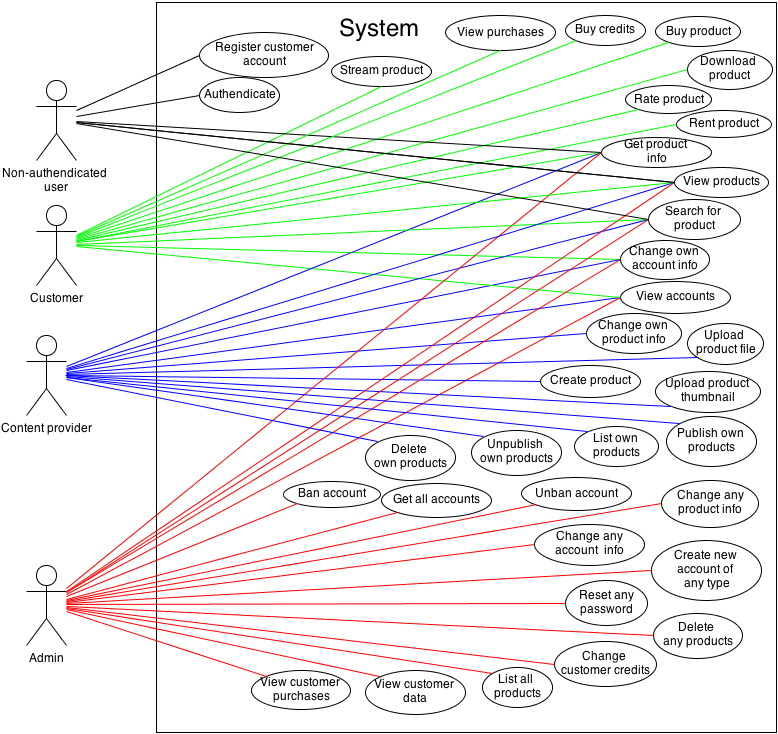
\includegraphics[scale=0.5]{illustrations/UseCaseDiagram.png}
\caption{Use case diagram for our web service}
\label{useCaseImg}
\end{figure}
\subsubsection{Requirements}
\label{s_serviceRequirements}
This section will focus on the requirements for the server. The following lists the non-functional requirements we have defined for the web services.

\begin{enumerate}[label=NFR-\arabic*]
	\item When put into production the server should have an uptime of at least 99 \% of planned uptime. Downtime, due to maintenance, must be announced at least 48 hours ahead.
	
	\item From the time a request has been received, to the time an answer has been sent, no more than 500 millisecond must have passed. Except when the answer contains a product-file (image, movie, video, etc.), in this case there is no deadline.
	
	\item All data (except the product-file itself) must be persisted for at least 5 years after it has gone out of usage (for legal reasons).
\end{enumerate}

The functional requirements for the server are derived from the use cases.

\newcounter{FR_Counter}

\begin{table}[H]
\centering
\caption{Functional requirements}
\label{functionalRequirements}
\begin{tabular}{|c|p{7cm}|p{0.5cm}|p{0.5cm}|p{0.5cm}|p{0.5cm}|}
\hline
ID & Description & NA & C & CP & A \\ \hline\hline
\refstepcounter{FR_Counter}FR-\arabic{FR_Counter} & Register new account & X & & & \\ \hline
\refstepcounter{FR_Counter}FR-\arabic{FR_Counter} & Authenticate & X & & & \\ \hline
\refstepcounter{FR_Counter}FR-\arabic{FR_Counter} & Get product information & X & X & X & X \\ \hline
\refstepcounter{FR_Counter}FR-\arabic{FR_Counter} & View products & X & X & X & X \\ \hline
\refstepcounter{FR_Counter}FR-\arabic{FR_Counter} & Search for products & X & X & X & X \\ \hline
\refstepcounter{FR_Counter}FR-\arabic{FR_Counter} & Buy products & & X & & \\ \hline
\refstepcounter{FR_Counter}FR-\arabic{FR_Counter} & Rent products & & X & & \\ \hline
\refstepcounter{FR_Counter}FR-\arabic{FR_Counter} & Rate products & & X & & \\ \hline
\refstepcounter{FR_Counter}FR-\arabic{FR_Counter} & Stream products & & X & & \\ \hline
\refstepcounter{FR_Counter}FR-\arabic{FR_Counter} & Download products & & X & & \\ \hline
\refstepcounter{FR_Counter}FR-\arabic{FR_Counter} & View purchases history &  & X &  &  \\ \hline
\refstepcounter{FR_Counter}FR-\arabic{FR_Counter} & Buy credits &  & X &  &  \\ \hline
\refstepcounter{FR_Counter}FR-\arabic{FR_Counter} & View accounts &  & X & X & X \\ \hline
\refstepcounter{FR_Counter}FR-\arabic{FR_Counter} & Change own account information & & X & X & X \\ \hline
\refstepcounter{FR_Counter}FR-\arabic{FR_Counter} & Upload product files & & & X & \\ \hline
\refstepcounter{FR_Counter}FR-\arabic{FR_Counter} & Create new products &  &  & X &  \\ \hline
\refstepcounter{FR_Counter}FR-\arabic{FR_Counter} & Upload product thumbnails &  &  & X &  \\ \hline
\refstepcounter{FR_Counter}FR-\arabic{FR_Counter} & Change informations about own products &  &  & X &  \\ \hline
\refstepcounter{FR_Counter}FR-\arabic{FR_Counter} & Publish own products &  &  & X &  \\ \hline
\refstepcounter{FR_Counter}FR-\arabic{FR_Counter} & Unpublish own products &  &  & X &  \\ \hline
\refstepcounter{FR_Counter}FR-\arabic{FR_Counter} & Delete own products &  &  & X &  \\ \hline
\refstepcounter{FR_Counter}FR-\arabic{FR_Counter} & List own products &  &  & X &  \\ \hline
\refstepcounter{FR_Counter}FR-\arabic{FR_Counter} & Change information about any product &  &  &  & X \\ \hline
\refstepcounter{FR_Counter}FR-\arabic{FR_Counter} & Change information about any account &  &  &  & X \\ \hline
\refstepcounter{FR_Counter}FR-\arabic{FR_Counter} & Get a list of all accounts &  &  &  & X \\ \hline
\refstepcounter{FR_Counter}FR-\arabic{FR_Counter} & Ban an account &  &  &  & X \\ \hline
\refstepcounter{FR_Counter}FR-\arabic{FR_Counter} & Unban an account &  &  &  & X \\ \hline
\refstepcounter{FR_Counter}FR-\arabic{FR_Counter} & Create new account of any type &  &  &  & X \\ \hline
\refstepcounter{FR_Counter}FR-\arabic{FR_Counter} & Reset any password &  &  &  & X \\ \hline
\refstepcounter{FR_Counter}FR-\arabic{FR_Counter} & Delete any product &  &  &  & X \\ \hline
\refstepcounter{FR_Counter}FR-\arabic{FR_Counter} & Change customer credits &  &  &  & X \\ \hline
\refstepcounter{FR_Counter}FR-\arabic{FR_Counter} & List all products &  &  &  & X \\ \hline
\refstepcounter{FR_Counter}FR-\arabic{FR_Counter} & View customer data &  &  &  & X \\ \hline
\refstepcounter{FR_Counter}FR-\arabic{FR_Counter} & View customer purchases &  &  &  & X \\ \hline
\refstepcounter{FR_Counter}FR-\arabic{FR_Counter} & Publish any products &  &  &  & X \\ \hline
\refstepcounter{FR_Counter}FR-\arabic{FR_Counter} & Unpublish any products &  &  &  & X \\ \hline
\refstepcounter{FR_Counter}FR-\arabic{FR_Counter} & Delete any products &  &  &  & X \\ \hline
\end{tabular}\\
\vspace{3mm}
NA = Non-authenticated, C = Customer, \\CP = Content provider, A = Admin
\end{table}
% !TeX spellcheck = en_US 
\subsubsection{Data Model}
When planning how to implement the server we had to decide on how to store our data. We had earlier decided to use MSSQL \textbf{[TODO: Den sætning virker underligt placeret? (K) ]}. To plan this we created a data model, see \fref{fig:datamodel}.
\begin{figure}[H]
  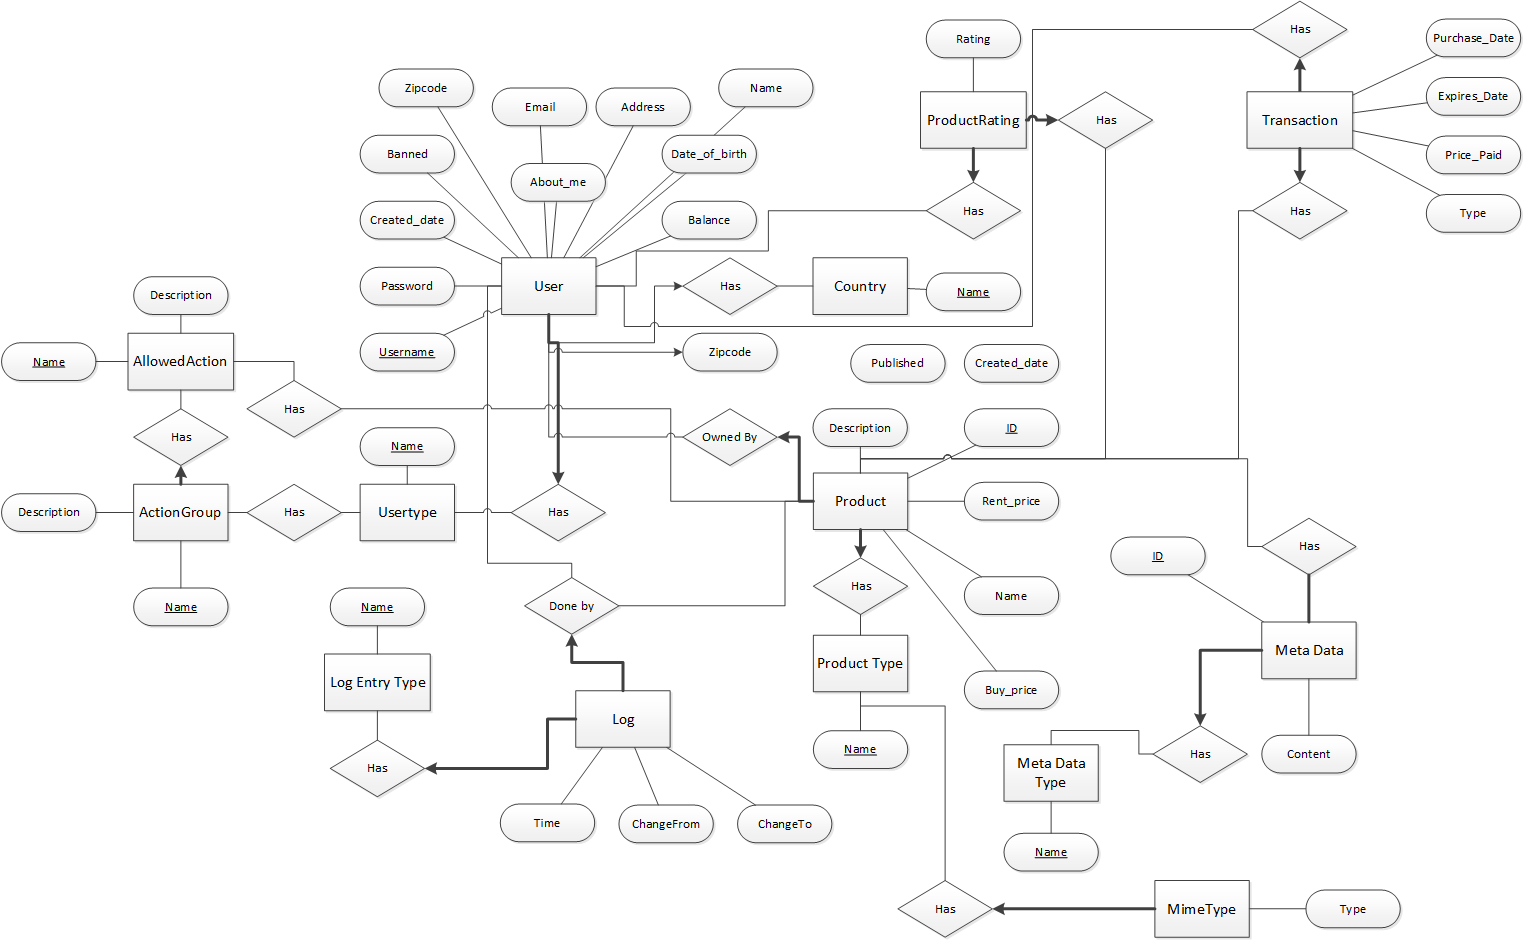
\includegraphics[width=\textwidth]{illustrations/Datamodel.png}
  \caption{Our data model as used by the database}
  \label{fig:datamodel}
\end{figure}
We will now explain the different entities, and their purpose in our program.

\begin{description}
\item[User] \hfill \\
Our first and possibly most important entity is the User entity. This contains all information regarding users of our system \todo{Everything here? Keep reading :)}{Krüger}. Each user also has a country, referenced through the Country entity explained later.

Furthermore, we have defined a user type for each user. This makes it possible to have all our users in one place, even if one is admin, and another one is a customer. We have created a separate entity for this; Usertype.

\item[Country] \hfill \\
Each user must have a country defined. The reason we modeled this as a separate entity is so that the user can select their country from a list of available ones.

\item[Usertype] \hfill \\
The user type defines which type the user has. The possible values in our program is:
\begin{itemize}
	\item Customer
	\item Content provider
	\item Admin
\end{itemize}

Each usertype has zero-to-many action groups. The function of that entity is explained later.

\item[ActionGroup] \hfill \\
An action group is a way to gather permissions in a group. This way we avoid having to give a lot of permissions to a user type. Our initial idea was to create action groups having names like `View general data', `Create and edit products' and `Administer products'. This would make it easy to create a new user type like `Content moderator' and assign permissions.

Our implementation was not like this though. We ended up making this entity completely useless as we created the exact same action groups as we had user types.

\item[AllowedAction] \hfill \\
Our AllowedAction entity is our way of defining permissions in the system. Whenever you need to check whether or not a user has permission to do something in our system you check the allowed action name (an example could be BAN\_UNBAN\_ANY).

The allowed action is referenced by both the ActionGroup entity and the Product entity. This is because we have chosen to model whether or not products should be buyable or rentable in our permissions system. Products can therefore have BUYABLE and RENTABLE allowed actions.

\item[Product] \hfill \\ 
Product is our main entity for storing movies, ebooks etc. It has some base information about products. It also has a product type. This is through the ProductType entity as described later.

There are three other entities that refer to Products.
\begin{itemize}
	\item MetaData
	\item ProductRating
	\item Transaction
\end{itemize}
All of which is described later.

\item[ProductType] \hfill \\
Each product has a product type. The product type is used to semantically separate the different types of products. Furthermore, it references another entity called MimeType.

\item[MimeType] \hfill \\
MimeType is used to limit which files can be uploaded for a specific product type. When creating a product you choose which type it is of. As it makes no sense to upload a PDF-file for a product of type `Movie' we chose to limit this using the information stored here.

\item[MetaData] \hfill \\
A product can have zero-to-many metadata attached. This can be used to describe things that are specific to the particular product. Like pages for an ebooks, length for a movie etc. Each metadata has a reference to the MetaDataType entity.

\item[MetaDataType] \hfill \\
The MetaDataType entity is used to control metadata. If users were to enter metadata, we would like to limit which type they could enter, to avoid things like `length', `Length', `LENgTh' and `Lengt' which are basically the same thing. It would also make search more versatile, as you, in theory, could search for movies with a length of over 1 hour.

\item[ProductRating] \hfill \\
This entity is used to store ratings that users have given products. Each user can only have one rating on each product. If a users tries to vote more than once, their vote should be updated.

We have defined ratings to be from -5 to 5. This means that user can be positive or negative towards a product.

\item[Transaction] \hfill \\
Our Transaction entity stores the purchases made. It records the information needed by our system for a purchase. If it is a rent the expire date is also stored here.

\item[Log] \hfill \\
While we planned our entire data model we wanted to make everything loggable. It is important to be able to monitor the system and the activity herein. Furthermore, our implementation would make it possible to revert things to previous states.

Each entry has a type, which is defined in the LogEntryType entity.

\item[LogEntryType] \hfill \\
This entity was planned to make searching through log entries easier. If we wanted to know how many people have logged in this year we could just take the log entries of type `login' and count them.
\end{description}
\subsubsection{Web Service API}
At the beginning of the process we appointed a single person to write a comprehensive API documentation for our web services.
The API should be able to handle all of the requirements agreed \todo{Upon}{Michael} with SMU.

The document was made available to SMU via Google Drive. From here the SMU group was able to add comments and ask questions about requests and their responses.

When parts of the API were approved by both ourselves and SMU the part was ready to be implemented as a web service.

Being as comprehensive as it is not only served as a users manual for SMU, \todo{Huh?}{Michael} but also as an implementation guide for us, since the API dictated every possible outcome for every request supported by each web service. After implementation it was additionally a perfect means of determining whether the implemented functionality was complete.

\subsubsubsection{How to read}
Each service is documented in the API documentation under the URI it uses. Following the URI is a description of the requests to this URI, a HTTP header template and a list of whom is able to perform the requests.

After this initial information, the actual format of the request follows. They are categorized in up to four kinds of requests that can be made to (almost) every service: GET, PUT, POST, and DELETE. \\
After the name of each request type, a description including request examples follows. \\
At the end of the examples a list of possible responses follows with explanation of what each response means.

For the complete API, see \apref{API_PDF}.
\subsubsection{Test Strategy}
When we started coding the server we did not have any idea of what or how we wanted to test, which made debugging very difficult. We used a lot of time on following calls through the different layers of the server to discover where an error or exception occurred. A few tests where made after most of the debugging had been done to prove that the server performed as wanted. That meant that we did not have a test strategy for the server.

A different approach to our solution could be that we in advance decided which parts of the server that we had to test and which parts where redundant to test. The level at which the tests should be made is the next to decide. When you make the tests, before the code to be tested or afterwards, is part of the test strategy as well.

The reason why we did not have any test strategy for the server, was not a conscious choice. We did not consider testing until most of the code had been written and debugged. Since we were lacking planning for the development we did not realize we had forgotten the testing. Not testing cost us more time than any test writing since the debugging was near impossible and very time consuming. By testing the individual parts of the server, we would have a much better idea of what kind of exception would be thrown from which part of the server. That in turn would make debugging much easier, since we would know where a exception would come from and we would most likely know why an exception is thrown. Using functions or types wrong would be discovered faster if we had tested the server more thoroughly, again since we would know it from the responses from the individual parts of the server. 
\newpage
% !TeX spellcheck = en_US
\subsection{Program Structure}
As mentioned our server is written in F\Sh which is a very powerful functional programming language with Types and parallel programming abilities. F\Sh can even be object oriented, but we have chosen not to use these abilities: We wanted the exercise of writing a fully functional system.

Our system is build of modules which are put together like bricks into layers that create a great structure. \textbf{[ TODO: Not quite satisfied with this formulation (M) ]}
\\We have an Outer Layer - or shell - which is the published Web Service. This layer is actually written in C\Sh.
\\Then we have a Checking Layer which uses a Permission Module to verify users and permissions before invoking functions deeper.
\\The Application Logic Layer is the actual working layer which has Account Module, Product Module and more.
\\The Persistence Layer is the lowest logical layer. It has the responsibility to create, save and update information on some sort of data storage.
\\Finally we have our Database in which we store our data.

Each Module can be replaced and the Checking Layer is entirely optional. For example one might want to change the Persistence Layer to persist against a file-system instead of a database, or one might want to do less or more extensive checks in the Checking Layer, without changing any of the other layers.

\subsubsubsection{Outer Layer}
We planned to write a thin C\Sh layer. The only responsibility for this layer would be to call the corresponding F\Sh functions. This, however, did not go as planned.

The layer ended up being responsible for receiving data, converting data and sending this to the F\Sh function. When data were to be extracted the layer was responsible for receiving data from F\Sh, converting data and sending it to the client.

This actually turned out to be okay, as we, in theory, could create a SOAP web service without any hassle, and we could possible extend it to different other services as well.
\subsubsubsection{Checking Layer}
Our checking layer is responsible for checking permissions on the users with the permissions. It could possibly do more than just check permissions.

We have created this layer, so that it can be removed without any functionality missing.
\subsubsubsection{Application Logic Layer}
In this layer we perform all our application logic. It is completely unaware of how data is stored however. Data selection and storage is handled elsewhere.
\subsubsubsection{Persistence Layer}
This layer is responsible for storing data. It has been made as generic as possible, so that if we chose to change storage to file instead it would be easy. It is also possible to easily implement a separate search-server if needed.

\begin{figure}[H]
  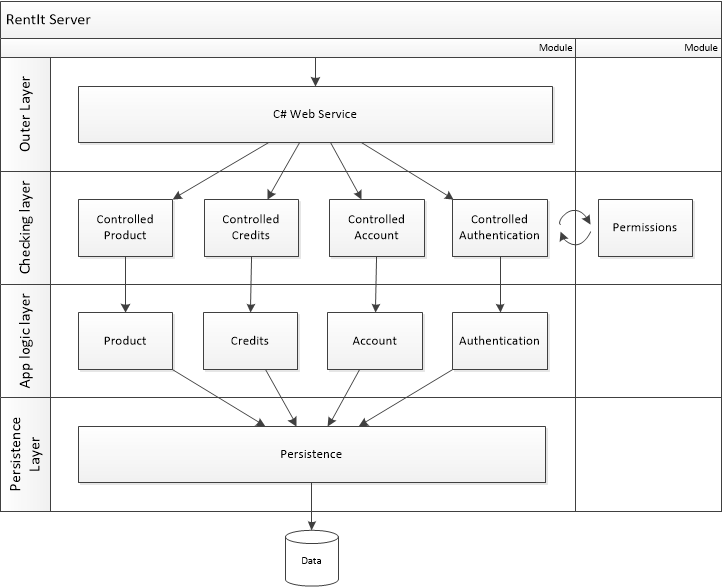
\includegraphics[width=\textwidth]{illustrations/ServerStructure.png}
  \caption{Our Server Structure}
  \label{fig:serverstructure}
\end{figure}
\newpage
\subsection{Quality Assurance}
This section documents the quality of our server implementation, points out bugs, missing functionality, and cases our services do not fulfill the requirements. \todo{and what?}{k}
\subsubsection{Fulfilling Requirements}
\label{serverfulfil}
The following section will briefly summarize if we have met our requirements, and in cases were we did not, explain why that is so.

Due to the fact that the web service is currently deployed at a server at ITU, together with the web services of all other groups, we have no real control over the server. The server seems to be heavily overloaded, and therefore our requirements concerning uptime and response time can not be met at all time.

Our requirement of persisting all data for a 5 year time period is also out of our reach, again due to the fact that we are only "guests" at the ITU server.

Regarding the functional requirements we have set up, we fulfil the requirements even though some user type have permission to more than the list expresses.
\textbf{[TODO: Gif example 'n explain this black magic for me!!! \\\textit{Please give this example and the explanation in a .gif animation. Best regards\\Dr. X :-)}]}\\
\textbf{[ TODO: Not enough? (M) ]}
\subsubsection{Testing}
We chose to divide the development of the server into two parts, the part responsible for account actions and the part responsible for product actions. \todo{Did we?}{Michael} During the development of the account part of the server, testing was primarily done by running the code when it became possible. The testing of the account module and controlled account module \todo{Only those two?}{Michael} was done by using the tool Fiddler2. This form of testing proved incredibly inefficient since we had no real idea of what kind of errors and exceptions the individual parts of the server threw and we could not test individual parts of the server to see if they independently responded correctly.

The second part of the development tests were written using FsUnit. It included testing of the product module, the credits module, and most of the account module. The tests mainly tested within the normal responses expected of the code and in some cases for some of the exceptions they throw. \todo{<-- Huh? Does not make sense.}{Philip} Since the debugging was mostly done by the time all of the tests were done it was primarily used to prove that the code performed as expected.

We have a total of 133 unit tests that all pass.
\subsubsection{Known Bugs}
From the first release of our server we have held a list of known bugs and a list of things yet not implemented. These were kept assure throughout the development process. \todo{What?}{Morten}
\\Here are the lists showing the current shortcomings of our server:
\subsubsubsection{Bug list}
\begin{itemize}
\item Adding metadata to products does not work.
\item Description string for products cannot pass more than 80 characters.
\item Deleting products not implemented.
\end{itemize}
The problem with the length of the description string, is a problem with our JSON serializer and should not take long to correct.
\subsubsubsection{To do}
\begin{itemize}
\item Handling metadata implemented, but not made available.
\item Somehow support deletion of products without robbing the customer of his purchase.
\item Correct product rating calculations.
\item Correct the improper detection of data too large to be handled by the database.
\item Implement ControlledProduct and ControlledCredits properly.
\end{itemize}
\subsubsubsection{Improvements}
While writing our client we discovered a number of things our server does not support which would have made it easier to write the client. There are also a couple of things we simply did not prioritize when we wrote the server.
\begin{itemize}
\item Encryption and security in general.
\item Simple web service methods such as a more specified method to get one or a few products.
\item A method for getting unpublished products for the Content Providers Dashboard.
\item Being able to limit the number of items returned from a service call.
\end{itemize}
\textbf{[ TODO: More? (C) ]}
\newpage
\subsection{Collaboration}
We started our collaboration with a short video conference where we introduced ourselves, agreed upon communication forms and planned weekly meetings. We also voiced our expectations of each other.
% !TeX spellcheck = en_US
\subsubsection{Communication}
For our collaboration we have used five technologies to communicate and share informations; three for communication and two for sharing information between the groups.

For sharing information we have used Dropbox and Google Drive. \vspace{-4mm}
\begin{description}
	\item Dropbox \\
		We chose to use Dropbox for sharing non-document files. We chose Dropbox since it is a program all of us already had installed, used before and are a very easy tool for sharing files which multiple people are not to change at the same time.
	\item Google Drive \\
		For files that multiple people might edit at the same time, and documents in general, we chose Google Drive, which allows for multiple people to edit the same file at the same time. Since everyone already had a Google Drive account it was easy to set up.
		Google Drive was mainly used for sharing the API documentation for the web service.
\end{description}

When communicating with SMU we used Skype, Google Hangout and email.
\vspace{-4mm}
\begin{description}
	\item Skype \\
		For most of our meetings with SMU we used Skype for video calls. Skype was a great improvement over the video conference tool used by ITU.
		Skype was also used as an instant message service, when small problems needed to be solved and questions answered. \\
		The drawback of using Skype as a video conference tool, is that when using the free plan (which we did), only two Skype accounts can be in a video conference at a time.
	\item Google Hangout \\
		If the group members of one of the groups where not able to meet at one place to conduct a video conference we used Google Hangout. With this tool up to 10 individual accounts can participate in one video conference at a time.
	\item Email \\
		To inform and communicate beside the video conferences the appointed liaisons emailed each other and passed the information on to the rest of their respective group.
		The use of email eliminated problems that might arise by different and unknown accents.
\end{description}
\subsubsection{Planning} % Planning hours?
\subsubsection{Matching Expectations}
We were very anxious to find out how dedicated and how much time our SMU group had for us and the project. It was very important for us to know. We were willing to lay a lot of hours into this interesting and rare opportunity to work in collaboration with a group of students from across the world, but only if they cared and were willing as well.

At our first meeting we set some expectations to each other. We were unsure about the affect the time difference would have on the response time. Without discussion we agreed upon a maximum of two days response time and 15 minutes of leeway upon agreed meeting times. Two days of response time is a very long time, and we voiced that we would not exceed 24 hours response time - they did not expect to do so either.

We were very happy with our SMU group and they did not break our contract. They exceeded our expectations in regard to the number of hours they put into the project and especially in regard to their initiative which was overwhelming. \todo {example perhaps?}{Morten}

We told our SMU group that we would like to be using REST ourselves (opposed to SOAP), but that we would offer SOAP as well if they preferred. They agreed to use REST without any questions.
\newpage
\subsection{Reflection (Server)}
Due to previous experiences we spent a lot of time on planning. Even then there are a lot of things we would like to do differently, were we given the chance to start over again.

We are very happy with our flexible design of layers and modules, but of course we want to make it even better and even less coupled next time. A major mistake of ours is the lack of design patterns throughout the server. When we review and debug our code, it proves to be more coupled than we intended. Being new to F\Sh and structuring code in a non object oriented manner, however, we are not completely sure what `design patterns' are available.

We wanted to create a logging feature where every module could report events and errors, but we never had the time. Writing the log might have saved us time. When debugging it was not always apparent which module failed or which module received faulty information. 

When writing the client, we encountered a surprising lack of functionality from our server - exactly what we had tried hard to avoid. It is, however, hard to foresee and write all functionality which will be needed in the future, and so the only way we could have done better was if we had developed the client and server in parallel or the client first \todo{Rephrase to something better.}{Philip}.
Unfortunately we were in a terrible lack of time and we kept our focus on the client and did not write any new services.

\subsection{Reflection (SMU Collaboration)}
We were excited about the project and we really hoped to get a group who were as engaged and enthusiastic about the project as we were - and luckily we did.

Our collaboration with our Singaporean group went very well - beyond all expectations really. We got the impression that they also enjoyed working with us. We have held many meetings and we chatted every day.

\todo{Is this not mentioned other place?}{Philip}
\newpage
\subsection{Conclusion}
Through this section of the report we have walked through the development of our server, beginning at our planning iteration, with use cases and data modeling, to a program structure walk-through, and on to the important quality assurance chapter, which includes fulfilling requirements, testing and a list of bugs, before we end up talking about our collaboration with SMU.

In the Requirements section, we list three none-functional requirements. Do to the combined load of the shared project server our uptime and response time requirements have not always been met.

We also list 18 functional requirements which we set with our SMU group. Our server live up to all of these and more.
\newpage
\section{Client}
\subsection{Planning}
\subsubsection{Requirements}
For the client we had the same functional requirements as we had for the web service, see \pref{s_serviceRequirements}.

Regarding non-functional requirements we only settled for a single requirement: From the time a request has been received to the time an response has been sent, no more than 1000 millisecond must have passed, except for product file requests, in which case the transfer only is required to have started.
\subsubsection{Use Cases}
w00t?

% !TeX spellcheck = en_US
\subsubsection{Test Strategy}
After we finished the server we changed a lot in how we would continue the project and one of these things were a test strategy for the client. After we designed the client's structure we agreed on which parts of the program we had to test and which parts where not as important to test. Since we had very limited time we did not write test classes for any views and the tests on the rest were minimum tests, where we tested expected results on normal behavior and on error handling of the server's errors. We chose to write the tests after the code, which made it easier to write the tests. We chose to use PHPunit as our testing framework.

This was a conscious choice, since we were focusing the remaining time on completing the project. Instead of writing the tests afterwards we could have made them in advance, which would have required more in the design phase, but would have given a clearer idea of how the code should react in certain situations.
\subsubsection{User Interface Design}
\newpage
\subsection{Program Structure}
We spent a long time planning the program structure before developing our client. We wanted to have a good plan in this part, contrary to the previous one.

We chose to use the MVC pattern for structuring our client. Furthermore it was divided up into modules, each responsible for their part. It made it easy to extend, or take modules out.

When a request is made for a page in our client, we find the module to use from the URI requested. The next argument in the URI is which method to invoke. In our variation of MVC we invoke the method requested in the modules default controller. This is then responsible for returning some renderable content which in our case is a widget.

Our implementation of the MVC pattern defines View a little different than traditionally. We have a single view in our entire system: the CommonView. What this does is create the header and footer, and put the page content in the middle. All other view in our system are widgets. A widget is an object that can be turned into some HTML. The base class of widget basically just forces subclasses to override the ToHtml method.

The widget structure is based on the composite pattern. A lot of the widgets can contain other widgets. Just like a lot of HTML elements can contain other HTML elements.

Our widget structure makes everything interchangeable, and easy to extend. It also helps us avoiding a lot of code duplication, as we define elements like the <div> a single place in the code. If we need to change the implementation of all wrappers on the site, we would only have to change it in one place.

Because of the composite structure and inheritance, we could completely avoid writing any HTML in the modules widgets. We would extend the base class needed (in most cases the Widget\_Wrapper that contains a list of widgets and wraps this in a <div> element). We would then create the structure needed for the particular widget in the constructor. And when the ToHtml-method was called on the Widget\_Wrapper, it calls the ToHtml-methods of all the children, and gathers the output. 

Our models work like in any other MVC application. In our case we have a web service to store our data, and the models operate on this.
	\newpage
\subsection{Quality Assurance}
In this section we will prove the quality of our client, list known bugs and explain why some requirements have not been met.
\subsubsection{Fulfilling Requirements}
Regarding the functional requirements, found in \pref{s_serviceRequirements}, we did not fulfill all of the requirements. This was mainly due to the fact that we did not have enough time at the end of the process and therefore choose to cut of some the functionality and focus on the report.

\textbf{[ TODO: List the requirements we did not meet. ]}
\subsubsection{Testing}
We decided to write PHPUnit tests for the controllers and models, while testing of the views would be done by blackbox testing. We tested normal behavior and the exception handling of the exception thrown by the server. This ensured that we had a much better idea of where any problems arose during debugging. Error messaging in PHP is known for being very limited. By having a good idea of how the individual parts behaved we saved time on the debugging, since we did not have to go through all the code involved in-depth to solve the problem.

Since much of what was tested on the widgets focused on the design, this was done by blackbox testing as we saw it as the only way to test it.

\todo{Seems unnecessary since much is repeated from the Test Strategy section. Remove repeated content and put rest into the Test Strategy section.}{Philip}
\subsubsection{Known Bugs}
Our web client has been in development till the end of this project. Now that we are at our deadline it is time to summarize the remaining items on our bug list and todo list:

\subsubsubsection{Bug list}
\begin{itemize}
\item \todo{Nothing?}{Claus}
\end{itemize}

\subsubsubsection{To do}
\begin{itemize}
\item Upload widget for upload of thumbnails and media
\item Search
\end{itemize}

\todo{All features which depend on missing server functionality are also on the to do}{Philip}
\todo{Which is what Philip?}{Claus}

\subsubsubsection{Improvements}
We are very happy with our client and its structure. It is extremely flexible and functionality can easily be added. We do not wish to refactor anything structural about the client at this time.

The performance of our client is generally very good. Our web service however lacks methods for getting a more specific subset of products, which means we some times have to request more products than we need and then filter them on the client, which impacts the performance of the site. This is evident on the pages listing multiple products.

There are a few things which are out of scope for this project that one would add to our client before making the client available for the public. Those things would be:
\begin{itemize}
\item Encryption and general security
\item Better error messages
\item Payment for credits
\item Commercials
\item Prettier styling
\end{itemize}
\todo{More?}{Claus}
\newpage
\subsection{Reflection}
Our work on the client has been focused and well executed. We planned to build the client in a cool widget-composite structure. We wrote a lot of structural code before finally being able to see the result of our hard work. It turned out even better than we had hoped. Whenever we wanted to add functionality it was always painless and much quicker to implement than one would think. If you were to add a new widget you should have knowledge of HTML, but you will rarely write any HTML. You add attributes to the widget and the HTML is generated for you. This also has the benefit of consistent code since it is generated alike for all widgets.

% Remove following?
A minor fault in our structure became apparent when we had an error somewhere in our code. Often the page would render blank and our server error log would complain about an error in a ToHtml-method, but not in which subclass of Widget the error roots. Usually this was no big problem since we knew which changes we had made since the last time it worked.

Working on the client was well structured. We used a backlog with all the items (mostly widgets) related to the client and report. Each item was described and estimated in hours. When a group member was done with one item he assigned himself to the next. The backlog gave us an overview of which items needed to be done, which was in progress, which was done and how many hours of work lay ahead of us. We used \url{www.Scrumwise.com}
\newpage
\subsection{Conclusion}
We wrote our client in object oriented PHP and our tests using PHPUnit. The client makes use of the web services described in the first part of this report.

We wanted to write an object oriented client which should be very easy to maintain and that is exactly what we did. A single view creates the web page and fills its content with a widget composite structure.

We did not have the time to fulfill all the requirements and use cases we had set for ourselves. Specifically we did not create a widget for uploading thumbnails and other media. Aside from that our client is functional and very usable. The following functionality is working as intended:
% Be aware: The following list is copied to the report Conclusion. Any changes should be synchronized.
\begin{itemize}
\item Create, view and edit accounts
\item Create, view and edit products
\item Buy credits (though they are free for now)
\item View and stream purchases
\item Buy, rent and rate products
\item Administrators can edit everything and create content provider and administrator accounts
\end{itemize}
\newpage
\section{Conclusion}
In this report we develop a number of web services and a matching client in form of a website. We wrote the server in F\Sh with a web service layer written in C\Sh. We wrote the client in PHP.

We set many requirements for our system and neither part fulfilled all of them due to lack of time.

We fulfill by far the majority of the requirements and we have shown that we can develop a web service and a matching client.

\subsubsubsection{Collaboration}
We had a successful collaboration with a Singaporean group. Lynette, Cai Ling and Celestine were as engaged and enthusiastic about the project as we were. We held two weekly meetings and we chatted daily.

\subsubsubsection{Process} 
In the first part of the project, we did not use any specific development method - we listed what needed to be done and then we worked it from the top. We often had to work more hours than we thought to keep the deadlines and it put us under a lot of stress.

For the second part of the project we decided to incorporate many SCRUM artifacts and it was of great advantage to us. At this point we were far behind our time schedule, but with help from SCRUM artifacts we could estimate the tasks at hand and thereby exclude less important tasks and we could schedule workdays with enough hours to get the job done.

We were terribly behind on our assignments and we did not have time to write a review of another groups report.
\newpage
\addcontentsline{toc}{section}{\hspace{17pt}Appendix} % Adds to the Table of contents
\section*{Appendix}
\renewcommand*\thesubsection{\Roman{subsection}} % Makes all subsections be listed with upper case roman numbers
-\subsection{Contribution List}
Claus: 
\begin{itemize}
	\item Server
	\begin{itemize}
		\item lol
	\end{itemize}
	\item Client
	\begin{itemize}
		\item lol
	\end{itemize}
	\item Report
	\begin{itemize}
		\item lol
	\end{itemize}
\end{itemize}
Philip:
\begin{itemize}
	\item Server
	\begin{itemize}
		\item lol
	\end{itemize}
	\item Client
	\begin{itemize}
		\item lol
	\end{itemize}
	\item Report
	\begin{itemize}
		\item lol
	\end{itemize}
\end{itemize} 
Michael: 
\begin{itemize}
	\item Server
	\begin{itemize}
		\item lol
	\end{itemize}
	\item Client
	\begin{itemize}
		\item lol
	\end{itemize}
	\item Report
	\begin{itemize}
		\item lol
	\end{itemize}
\end{itemize}
Morten: 
\begin{itemize}
	\item Server
	\begin{itemize}
		\item lol
	\end{itemize}
	\item Client
	\begin{itemize}
		\item lol
	\end{itemize}
	\item Report
	\begin{itemize}
		\item lol
	\end{itemize}
\end{itemize}
Nicolai: 
\begin{itemize}
	\item Server
	\begin{itemize}
		\item lol
	\end{itemize}
	\item Client
	\begin{itemize}
		\item lol
	\end{itemize}
	\item Report
	\begin{itemize}
		\item lol
	\end{itemize}
\end{itemize}
\newpage
\subsection{Use cases}
\label{Apendix_usecases}
\textbf{Success scenario: Register new user} \\
Jane Doe wants to register and become a customer. 
\begin{tabbing}
\hspace{5mm}\=\hspace{28mm}\=\kill
\>Primary Actor:\> Non-registered user\\
\>Precondition:\> -\\
\>Postcondition:\> A new customer account is created, and the user is logged in.
\end{tabbing}
\begin{enumerate} \setlength{\itemsep}{-1mm}
	\item Jane Doe clicks the 'register' link.
	\item Jane Doe enters the required information (email, username and password).
	\item Jane Doe submits the request.
\end{enumerate}
% % %
\vspace{3mm}
\textbf{Success scenario: Show product} \\
Jane Doe wants see what products there are available of the type 'ebook'.
\begin{tabbing}
\hspace{5mm}\=\hspace{26mm}\=\kill
\>Primary Actor:\> Any\\
\>Precondition:\> -\\
\>Postcondition:\> -
\end{tabbing}
\begin{enumerate} \setlength{\itemsep}{-1mm}
	\item Jane Doe clicks the browse products link.
	\item She clicks more in the box containing ebooks.
	\item She is presented with all the products of type ebook.
\end{enumerate}
% % %
\vspace{3mm}
\textbf{Success scenario: Manage account} \\
John Doe wants to edit his account information.
\begin{tabbing}
\hspace{5mm}\=\hspace{26mm}\=\kill
\>Primary Actor:\> Customer or Content Provider\\
\>Precondition:\> The actor is logged in.\\
\>Postcondition:\> The actor has changed his account information.
\end{tabbing}
\begin{enumerate} \setlength{\itemsep}{-1mm}
	\item John Doe goes to his account-page.
	\item John Doe changes the data his wishes to be changed.
	\item John Doe clicks the 'save' link.
\end{enumerate}
% % %
\vspace{3mm}
\textbf{Success scenario: Log in} \\
John Doe wants to log in to his account. 
\begin{tabbing}
\hspace{5mm}\=\hspace{26mm}\=\kill
\>Primary Actor:\> Not authenticated\\
\>Precondition:\> The actor already has an account.\\
\>Postcondition:\> The actor is logged in.
\end{tabbing}
\begin{enumerate} \setlength{\itemsep}{-1mm}
	\item John Doe click on the 'log in' link.
	\item John Doe enters his login information (username and password).
	\item John Doe clicks the 'enter' link.
\end{enumerate}
% % %
\vspace{3mm}
\textbf{Success scenario: Rent product} \\
Spiderman wants to rent the movie 'The Dark Knight Rises'. 
\begin{tabbing}
\hspace{5mm}\=\hspace{26mm}\=\kill
\>Primary Actor:\> Customer\\
\>Precondition:\> The actor is logged in and it is possible to rent the product.\\
\>Postcondition:\> The actor has rented the product and the credits\\ \hspace{85px} is withdrawn from the actor's account.
\end{tabbing}
\begin{enumerate} \setlength{\itemsep}{-1mm}
	\item Spiderman navigates to the movie.
	\item He clicks the 'rent product' link.
\end{enumerate}
% % %
\vspace{3mm}
\textbf{Success scenario: Create new product} \\
Claus wants to create a new product. 
\begin{tabbing}
\hspace{5mm}\=\hspace{26mm}\=\kill
\>Primary Actor:\> Content Provider\\
\>Precondition:\> The actor is logged in.\\
\>Postcondition:\> The actor has created a new unpublished product\\ \hspace{85px} without an associated media file.
\end{tabbing}
\begin{enumerate} \setlength{\itemsep}{-1mm}
	\item Claus clicks the 'Create product' link.
	\item He enters the requested data.
	\item He clicks the 'create' link.
\end{enumerate}
% % %
\vspace{3mm}
\textbf{Success scenario: Add media to a product} \\
Claus wants to add a movie to his newly created product.
\begin{tabbing}
\hspace{5mm}\=\hspace{26mm}\=\kill
\>Primary Actor:\> Content Provider\\
\>Precondition:\> The actor is logged in and has a product without any\\ \hspace{85px} media.\\
\>Postcondition:\> The actor has uploaded the media and the product is\\ \hspace{85px} published.
\end{tabbing}
\begin{enumerate} \setlength{\itemsep}{-1mm}
	\item Claus navigates to the product.
	\item He clicks the 'add media' link.
	\item He chooses the media from his computer and clicks the 'upload' link.
\end{enumerate}
% % %
\vspace{3mm}
\textbf{Success scenario: Edit product information} \\
Claus wants to edit information about one of his products.
\begin{tabbing}
\hspace{5mm}\=\hspace{26mm}\=\kill
\>Primary Actor:\> Content Provider or Admin\\
\>Precondition:\> The actor is logged in. If actor is a Content Provider, he\\ \hspace{85px} needs to own the product.\\
\>Postcondition:\> The actor has changed the information about the product.
\end{tabbing}
\begin{enumerate} \setlength{\itemsep}{-1mm}
	\item Claus navigates to the product he wants to change.
	\item He changes the information.
	\item He clicks the 'save' link.
\end{enumerate}
% % %
\vspace{3mm}
\textbf{Success scenario: Unpublish a product} \\
Claus wants to unpublish one of his products.
\begin{tabbing}
\hspace{5mm}\=\hspace{26mm}\=\kill
\>Primary Actor:\> Content Provider or Admin\\
\>Precondition:\> The actor is logged in and the product has to be published. If the actor is a\\ \hspace{85px} Content Provider, he needs to own the product.\\
\>Postcondition:\> The product is unpublished.
\end{tabbing}
\begin{enumerate} \setlength{\itemsep}{-1mm}
	\item Claus navigates to the product he wants to unpublish.
	\item He clicks the 'unpublish' link.
\end{enumerate}
% % %
\vspace{3mm}
\textbf{Success scenario: Publish a product} \\
Claus wants to publish one of his products.
\begin{tabbing}
\hspace{5mm}\=\hspace{26mm}\=\kill
\>Primary Actor:\> Content Provider or Admin\\
\>Precondition:\> The actor is logged in and the product has to be\\ \hspace{85px} unpublished and be associated with a media. If the actor is a Content Provider, he needs to own the product.\\
\>Postcondition:\> The product is published.
\end{tabbing}
\begin{enumerate} \setlength{\itemsep}{-1mm}
	\item Claus navigates to the product he wants to publish.
	\item He clicks the 'publish' link.
\end{enumerate}
% % %
\vspace{3mm}
\textbf{Success scenario: Change information about a specific Customer, Content Provider or Admin} \\
Morten wants to change Spiderman's account information.
\begin{tabbing}
\hspace{5mm}\=\hspace{26mm}\=\kill
\>Primary Actor:\> Admin\\
\>Precondition:\> The actor is logged in.\\
\>Postcondition:\> The actor has changed the information about the account.
\end{tabbing}
\begin{enumerate} \setlength{\itemsep}{-1mm}
	\item Morten navigates to Spiderman's profile-page.
	\item He make the wanted changes.
	\item He clicks the 'save' link.
\end{enumerate}
% % %
\vspace{3mm}
\textbf{Success scenario: Ban a specific account} \\
Morten wants to ban Claus's account.
\begin{tabbing}
\hspace{5mm}\=\hspace{26mm}\=\kill
\>Primary Actor:\> Admin\\
\>Precondition:\> The actor is logged in, the other actor is not already banned,\\ \hspace{85px} neither is the account in question the admin himself.\\
\>Postcondition:\> The actor has banned the account in question.
\end{tabbing}
\begin{enumerate} \setlength{\itemsep}{-1mm}
	\item Morten navigates to Claus' profile-page.
	\item Morten clicks the 'ban' link.
\end{enumerate}
% % %
\vspace{3mm}
Morten wants to unban Claus' account.
\begin{tabbing}
\hspace{5mm}\=\hspace{26mm}\=\kill
\>Primary Actor:\> Admin\\
\>Precondition:\> The actor is logged in, the other actor is banned, and the\\ \hspace{85px} account in question is not the admin himself.\\
\>Postcondition:\> The actor has unbanned the account in question.
\end{tabbing}
\begin{enumerate} \setlength{\itemsep}{-1mm}
	\item Morten navigates to Claus' profile-page.
	\item Morten clicks the 'unban' link.
\end{enumerate}
% % %
\vspace{3mm}
\textbf{Success scenario: Create new account} \\
Morten wants to create a new account.
\begin{tabbing}
\hspace{5mm}\=\hspace{26mm}\=\kill
\>Primary Actor:\> Admin\\
\>Precondition:\> The actor is logged in.\\
\>Postcondition:\> A new account is created.
\end{tabbing}
\begin{enumerate} \setlength{\itemsep}{-1mm}
	\item Morten opens the 'create new account' page.
	\item Morten fills in the form.
	\item He clicks the 'save' link.
\end{enumerate}
% Following should be added as inputs
\subsection{Review Report}
\subsection{SMU Wiki}
\newpage
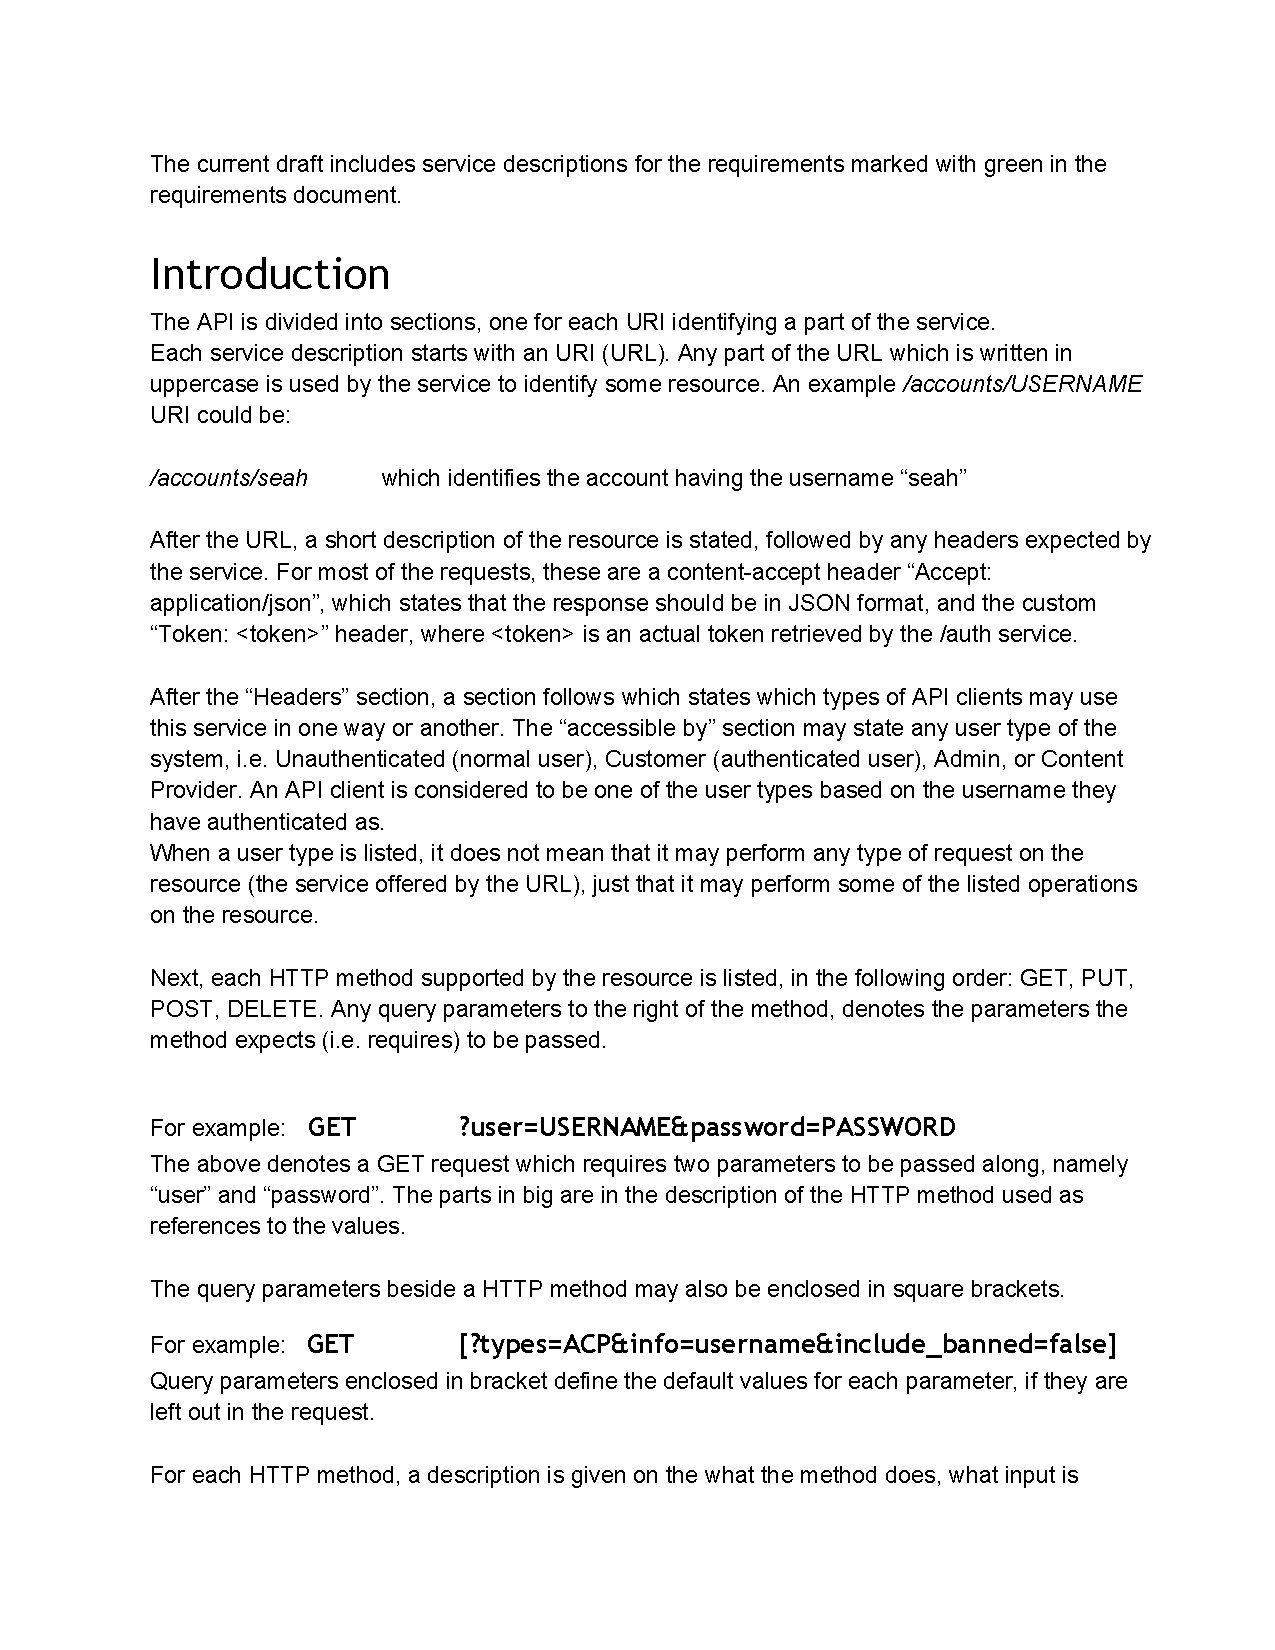
\includepdf[scale=0.8,pagecommand={\subsection{Web service API}\label{API_PDF}},pages=1]{texts/Appendix/API.pdf}
\includepdf[scale=0.8,pagecommand={},pages=2-]{texts/Appendix/API.pdf}

% Add bibliography
\bibliographystyle{cell}
\bibliography{bib}
\end{document}